\begin{yl}{3}{Paberi voltimine}{volt}{1 sekund}{30 punkti}
  \emph{Idee ja teostus: Targo Tennisberg, lahenduse selgitus: Ahto Truu}

  Nagu tekstis juba vihjatud, on selles ülesandes kaks põhimõtteliselt erinevat juhtu: kas murdejoon on paralleelne ruutude külgede või diagonaalidega.

  Ruutude külgedega paralleelne joon omakorda võib olla horisontaalne või vertikaalne:
  \begin{center}
  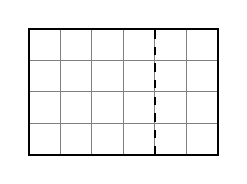
\begin{tikzpicture}[scale=0.4]
    \draw[gray] (0, 0) grid (6, 4);
    \draw[thick] (0, 0) rectangle (6, 4);
    \draw[thick, dashed] (4, 0) -- (4, 4);
  \end{tikzpicture}
  \hspace{1cm}
  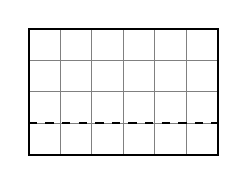
\begin{tikzpicture}[scale=0.4]
    \draw[gray] (0, 0) grid (6, 4);
    \draw[thick] (0, 0) rectangle (6, 4);
    \draw[thick, dashed] (0, 1) -- (6, 1);
  \end{tikzpicture}
  \end{center}

  Mõlemal juhul määrab vastuse suurem neist kahest ristkülikust, milleks murdejoon algse paberi jagab.

  Vertikaalse murdejoone tunneme ära sellest, et $X_1 = X_2$ (lisaks teame, et $Y_1$ ja $Y_2$ on sel juhul kindlasti kas $0$ ja $N$ või $N$ ja $0$). Siis on tulemuse kõrgus $N$ ja laius $\max(X_1, M - X_1)$.

  Sarnaselt on horisontaalse murdejoone tunnuseks $Y_1 = Y_2$ ning tulemuseks saadava ristküliku laius $M$ ja kõrgus $\max(Y_1, N - Y_1)$.

  Diagonaalse murdejoone puhul võivad selle otspunktid olla kas naaberkülgedel (alloleval joonisel vasakul) või vastaskülgedel (alloleval joonisel paremal):
  \begin{center}
  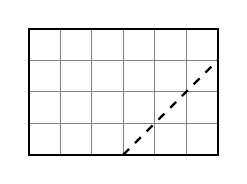
\begin{tikzpicture}[scale=0.4]
    \draw[gray] (0, 0) grid (6, 4);
    \draw[thick] (0, 0) rectangle (6, 4);
    \draw[thick, dashed] (3, 0) -- (6, 3);
  \end{tikzpicture}
  \hspace{1cm}
  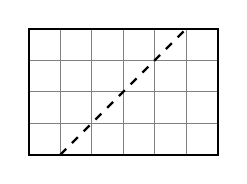
\begin{tikzpicture}[scale=0.4]
    \draw[gray] (0, 0) grid (6, 4);
    \draw[thick] (0, 0) rectangle (6, 4);
    \draw[thick, dashed] (1, 0) -- (5, 4);
  \end{tikzpicture}
  \end{center}

  Võib tunduda, et siin on palju võimalikke variante, mida peaks kõiki eraldi käsitlema, aga osutub, et vastus on kõigil neil juhtudel leitav täpselt sama meetodiga!

  \begin{center}
  \begin{tikzpicture}[scale=0.4]
    \draw[gray] (0, 0) grid (6, 4);
    \draw[thick] (0, 0) -- (3, 0) -- (6, 3) -- (6, 4) -- (0, 4) -- cycle;
    \draw[thick, dashed, pattern=north west lines] (3, 0) -- (3, 3) -- (6, 3) -- cycle;
  \end{tikzpicture}
  \hspace{1cm}
  \begin{tikzpicture}[scale=0.4]
    \draw[gray] (0, 0) grid (6, 4);
    \draw[gray] (1, 4) grid (5, 5);
    \draw[thick] (0, 0) -- (1, 0) -- (5, 4) -- (5, 5) -- (1, 5) -- (1, 4) -- (0, 4) -- cycle;
    \draw[thick, dashed, pattern=north west lines] (1, 0) -- (1, 4) -- (5, 4) -- cycle;
  \end{tikzpicture}
  \end{center}

  Kui murdejoone otspunktid on naaberkülgedel, siis saab kahekordselt kaetud täisnurkse kolmnurga kujuline ala, mille laius on $|X_1 - X_2|$ ja kõrgus $|Y_1 - Y_2|$ (viirutatud ala ülaloleval joonisel vasakul) ja tulemuseks saadava kujundi pindala on algsest paberist selle võrra väiksem.

  Ülesande arvatavasti raskeim osa on märgata, et ka vastaskülgedel olevate otspuktidega murdjoone korral saab kahekordselt kaetud samasugune kolmnurk (ülaloleval joonisel paremal).

  Kõiki neid tähelepanekuid kombineerides on lahenduse sisuline osa lõpuks 3-realine:
  \begin{lstlisting}[language=Python]
  def area(m, n, x1, y1, x2, y2):
    if x1 == x2: return max(m - x1, x1) * n
    if y1 == y2: return max(n - y1, y1) * m
    return m * n - abs((x1 - x2) * (y1 - y2) / 2)
  \end{lstlisting}

  \clearpage
  Tehniline detail C++ kasutajatele: kui \lstinline[language=C++]{x1} ja \lstinline[language=C++]{x2} on täisarvutüüpi, siis on seda ka \lstinline[language=C++]{x1-x2}; kui \lstinline[language=C++]{x1-x2} ja \lstinline[language=C++]{y1-y2} on täisarvutüüpi, siis on seda ka \lstinline[language=C++]{(x1-x2)*(y1-y2)}; ja siis on ka jagamine \lstinline[language=C++]{(x1-x2)*(y1-y2)/2} täisarvuline ning viskab vastuse murdosa minema. Selle vältimiseks võib:
  \begin{xitem}
    \item kirjutada jagaja reaalarvuna: \lstinline[language=C++]{(x1-x2)*(y1-y2)/2.0} või
    \item teisendada jagatava enne jagamist reaalarvuks: \lstinline[language=C++]{double((x1-x2)*(y1-y2))/2}.
  \end{xitem}
  Teisel juhul on sulgude paigutus väga oluline! Avaldis \lstinline[language=C++]{double((x1-x2)*(y1-y2)/2)} teeb kõigepealt täsarvulise jagamise (koos murdosa äraviskamisega) ja teisendab siis selle tulemuse reaalarvutüüpi; juba minema visatud murdosa see enam tagasi ei too.
\end{yl}
